82. $y=\cfrac{|x-1|}{x-1}(x^2-4)=\begin{cases}x^2-4,\ x>1\\ 4-x^2,\ x<1.\end{cases}$
$$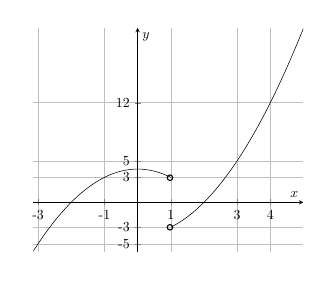
\begin{tikzpicture}[scale=0.5]
\begin{axis}[
    axis lines = middle,
    grid=major,
    legend pos={south west},
    xlabel = {$x$},
    ylabel = {$y$},
    ymin=-6,
    ymax=21,
    xtick={-3,-1,1,3,4},
    xticklabels={-3,-1,1,3,4},
    ytick={-5,-3, 3,5,12},
    yticklabels={-5,-3, 3,5,12}            ]
	\addplot[domain=-4:1, samples=100, color=black] {4-x*x};
\addplot[domain=1:6, samples=100, color=black] {x*x-4};
%\addplot[domain=-3.1:2.5, samples=100, color=red] {70*abs(1-2*abs(abs(x)-2))-10*x^2+10*x-70};
	%\addlegendentry{$\text{Рис. 1}$};
\end{axis}
\draw (3.47,1.89) circle (2pt);
\draw (3.47,0.63) circle (2pt);
\end{tikzpicture}$$
